\chapter{Étude détaillée du projet}
\par Ce chapitre est consacré à la description de l'aspect fonctionnel du cycle de développement à travers l'analyse de l'existant, le diagramme des cas d'utilisation et le détail des objectifs techniques fixés pour le projet.


\clearpage
\section{Introduction}
Après avoir défini les objectifs du projet dans le chapitre précédent, nous allons maintenant nous concentrer sur la spécification précise des besoins fonctionnels et non fonctionnels. Cette étape est essentielle pour s'assurer que le système répondra aux attentes des utilisateurs et aux exigences de la Digital Factory. Nous procéderons à une analyse approfondie des fonctionnalités requises, en identifiant les interactions entre les acteurs et le système. \\
Nous examinerons également les contraintes et les exigences non fonctionnelles auxquelles le système doit se conformer. Cette étude détaillée servira de base solide pour la conception de l'architecture du système, qui sera présentée dans les chapitres ultérieurs. Grâce à cette analyse approfondie, nous serons en mesure de proposer une solution optimale qui répondra aux besoins identifiés et garantira la satisfaction des utilisateurs.

\section{Analyse de l'existant}
\subsection{Étude de l'existant}
Dans le cadre de sa stratégie de digitalisation, l'équipe de développement de la Digital Factory au sein de la Société Générale ABS a mis en place une solution web et mobile appelée SG CONNECT. Cette application a été développée dans le but de simplifier, accélérer et sécuriser la gestion des comptes clients en offrant une gamme variée de services bancaires à distance, accessibles 24 heures sur 24 et 7 jours sur 7. Cette solution unique a été déployée pour desservir les 14 filiales de la zone AFMO (Afrique Méditerranée et Outre-mer).\\

SG CONNECT a été conçue pour remplacer les applications existantes telles que Cadinet et Mobilize, ou pour répondre directement aux besoins croissants en matière de services bancaires à distance. Actuellement, l'application est disponible pour les filiales suivantes : Burkina Faso, Madagascar, Mauritanie, Congo, Tchad, Bénin, Côte d'Ivoire, Guinée, Cameroun, Sénégal et Ghana.\\

Dans sa version R2+ actuelle, l'application SG CONNECT propose plusieurs fonctionnalités, dont :

\begin{itemize}
    \item[•] Téléchargement du RIB et des relevés de compte
    \item[•] Localisation des agences et des distributeurs automatiques de billets à proximité
   \item[•] Mode démo
   \item[•] Autres options : CGU \& FAQ et À propos
   \item[•] Consultation des comptes
   \item[•] Gestion des mots de passe : récupération d'un mot de passe oublié et changement de mot de passe
   \item[•] Consultation du taux de change
   \item[•] Graphiques représentant les données financières
   \item[•] Consultation des crédits et placements
   \item[•] Virements compte à compte et virements vers bénéficiaires SG et Confrères
   \item[•] Gestion des bénéficiaires
   \item[•] Recherche dans l'historique des opérations
   \item[•] Historique des virements
   \item[•] Commande de chéquier
  \item[•]  Simulateur de crédit
   \item[•] Souscription à distance
   \item[•] Paramétrage de la langue
   \item[•] Virement Wallet
   \item[•] Gestion des Alias et jauge de solde
   \item[•] Gestion des bénéficiaires Wallet
   \item[•] Gestion des impayés de crédits
   \item[•] Édition du reçu de virement
   \item[•] Affichage des libellés structurés
   \item[•] Contactez-nous
   \item[•] Gestion des alertes
   \item[•] Virement intrarégional
   \item[•] Virement interopérable
   \item[•] Authentification par biométrie et empreinte digitale
   \item[•] Notifications PUSH\\
\end{itemize}

Cependant, il est important de souligner que l'application SG CONNECT repose sur une infrastructure backend solide et sécurisée. Dans ce contexte, la Digital Factory a créé la plateforme digitale UNIBANK pour répondre aux exigences de l'Open Banking et garantir la sécurité et le consentement des clients dans le partage de leurs données financières. UNIBANK est une plateforme d'Open Banking qui ouvre le système d'information de la Société Générale et facilite l'échange sécurisé de données avec des tiers.\\

UNIBANK joue un rôle essentiel en assurant la connectivité et l'interopérabilité entre les applications consommatrices, telles que SG CONNECT, et les APIs développées, en masquant la complexité technique et en garantissant le respect des réglementations sécuritaires. La plateforme UNIBANK est construite sur une technologie open-source appelée WSo2 et comprend plusieurs projets (squads) travaillant sur les différentes couches et briques de son architecture pour assurer la disponibilité et la sécurité des APIs consommées.\\

Ainsi, SG CONNECT constitue l'interface conviviale et intuitive pour les clients, leur offrant un accès facile à une large gamme de services bancaires. En arrière-plan, UNIBANK fournit les fonctionnalités backend et la connectivité nécessaire pour garantir une expérience utilisateur optimale et sécurisée.

\subsection{Limitations de l'existant}
L'application SG CONNECT, bien qu'elle propose déjà un ensemble de fonctionnalités bancaires à distance, présente certaines limitations qui restreignent l'expérience utilisateur et les services offerts. Parmi les principales limitations identifiées, on peut citer l'absence d'affichage des cartes monétiques associées aux comptes des clients, ce qui limite la visibilité et le suivi des transactions liées à ces cartes. De plus, les informations sur les plafonds nationaux et internationaux de chaque carte ne sont pas disponibles, rendant difficile pour les clients de gérer et contrôler leurs dépenses selon leurs besoins spécifiques. De plus, l'application ne fournit pas de visibilité claire sur les produits souscrits par le client pour chaque compte bancaire, ce qui limite la compréhension globale de la situation financière.\\

Ces limitations ont un impact sur l'expérience utilisateur et empêchent les clients d'accéder à des informations cruciales pour gérer efficacement leurs comptes et effectuer des transactions en toute confiance. 

\section{Analyse et identification des besoins}
\subsection{Besoins fonctionnels}
Afin d'atteindre les objectifs souhaités, il est crucial d'identifier avec précision les besoins fonctionnels et non fonctionnels du projet. Les différentes réunions de Backlog Grooming ont permis de spécifier en détail les exigences fonctionnelles que la solution doit satisfaire. L'ensemble de la solution doit répondre aux spécifications fonctionnelles suivantes :

\begin{itemize}
    \item[•] \textbf{Affichage des cartes monétiques :} L'application doit permettre aux utilisateurs de visualiser toutes leurs cartes monétiques associées à leurs comptes bancaires, avec des informations détaillées telles que le type de carte, le numéro de carte et la date d'expiration.
    \item[•] \textbf{Suivi des transactions liées aux cartes :} Les utilisateurs doivent pouvoir consulter l'historique complet des transactions effectuées avec chaque carte monétique, afin de pouvoir vérifier les dépenses, détecter les transactions suspectes et suivre l'utilisation de leurs cartes.
    \item[•] \textbf{Consultation des plafonds nationaux et internationaux :} Les utilisateurs doivent avoir accès aux plafonds de dépenses nationaux et internationaux de chaque carte monétique, leur permettant ainsi de gérer et d'ajuster leurs limites de dépenses en fonction de leurs besoins spécifiques.
    \item[•] \textbf{Consulter un store de produits bancaires :} Les utilisateurs doivent pouvoir accéder à un store intégré dans l'application qui présente une gamme de produits bancaires disponibles, tels que des prêts, des cartes de crédit ou des comptes d'épargne.
    \item[•] \textbf{Consulter le descriptif d'un produit :} L'application doit permettre aux utilisateurs de consulter les détails et les caractéristiques spécifiques de chaque produit bancaire présenté dans le store, afin de prendre des décisions éclairées lors de leur choix.
    \item[•] \textbf{Appliquer les différents contrôles d'éligibilité :} Lorsqu'un utilisateur sélectionne un produit bancaire dans le store, l'application doit effectuer automatiquement les vérifications d'éligibilité requises, en fonction des critères prédéfinis, pour déterminer si l'utilisateur remplit les conditions nécessaires pour souscrire à ce produit.
    \item[•] \textbf{Envoyer un SMS avec code de confirmation :} Pour les transactions sensibles ou les opérations nécessitant une vérification supplémentaire, l'application doit être en mesure d'envoyer un SMS contenant un code de confirmation au numéro de téléphone mobile enregistré par l'utilisateur.
    \item[•] \textbf{Envoyer un mail de confirmation :} Après la réalisation d'une transaction ou l'accomplissement d'une opération importante, l'application doit envoyer un courrier électronique de confirmation à l'adresse e-mail associée au compte de l'utilisateur pour lui fournir une trace écrite de la transaction effectuée.
    \item[•] \textbf{Visibilité des produits souscrits par le client :} L'application doit fournir aux utilisateurs des informations détaillées sur les produits bancaires souscrits pour chaque compte, comme les crédits, les prêts ou les services d'investissement, leur permettant de mieux gérer leurs engagements financiers.
    \item[•] \textbf{Disponibilité en deux versions de langues :} Toutes les fonctionnalités mentionnées ci-dessus doivent être disponibles en français et en anglais afin de répondre aux besoins des utilisateurs francophones et anglophones et de garantir une expérience utilisateur fluide et personnalisée, quel que soit la langue choisie par l'utilisateur.
\end{itemize}

\subsection{Besoins non fonctionnels}
Avant de présenter le diagramme de cas d'utilisation, il est essentiel de mettre en évidence les besoins non fonctionnels. Ces besoins représentent les contraintes auxquelles le système est soumis pour sa réalisation et son bon fonctionnement. Ils doivent être pris en compte tout au long du développement du projet afin de garantir la performance du produit final et de satisfaire les exigences de la Digital Factory ainsi que les attentes des clients. Les contraintes suivantes ont été identifiées :

\begin{itemize}
    \item[•] \textbf{Performance :}  Le système doit être réactif et offrir des temps de réponse rapides, afin de permettre aux utilisateurs d'accéder aux fonctionnalités et d'effectuer leurs opérations bancaires de manière fluide et sans délai notable.
    \item[•] \textbf{ Sécurité :} La sécurité des données et des transactions est primordiale. Le système doit mettre en place des mesures de sécurité robustes pour protéger les informations sensibles des utilisateurs, telles que les données personnelles, les identifiants de connexion et les détails financiers.
    \item[•] \textbf{Disponibilité :} Le système doit être disponible en permanence, avec un temps d'indisponibilité minimal prévu pour les opérations de maintenance planifiées. Cela garantit que les utilisateurs peuvent accéder à leurs comptes et effectuer des transactions à tout moment, sans interruption majeure du service.
    \item[•] \textbf{Évolutivité :} Le système doit être conçu de manière à pouvoir s'adapter et évoluer avec les besoins futurs. Il doit être extensible pour prendre en charge de nouvelles fonctionnalités, des volumes de données croissants et une augmentation du nombre d'utilisateurs.
    \item[•] \textbf{Convivialité :} L'interface utilisateur doit être conviviale et intuitive, permettant aux utilisateurs de naviguer facilement dans l'application, de comprendre les fonctionnalités offertes et d'effectuer leurs actions sans difficulté. Une attention particulière doit être accordée à l'ergonomie, à la lisibilité des textes et aux indications visuelles pour guider les utilisateurs.
    \item[•] \textbf{Interopérabilité :} Le système doit être compatible avec d'autres systèmes et services existants au sein de la Société Générale ou avec des partenaires externes. Cela facilite l'intégration avec d'autres applications et assure une communication fluide et sécurisée des données entre les différents systèmes.
\end{itemize}


\section{Diagramme de cas d'utilisation}
Chaque interaction du client avec le système est représentée par un cas d'utilisation. Chaque cas d'utilisation décrit une fonctionnalité ou une action spécifique que le client peut effectuer dans le système pour atteindre un résultat attendu. Le diagramme de cas d'utilisation illustre les différentes fonctionnalités offertes au client et montre comment celles-ci répondent à ses besoins.\\

Voici le diagramme de cas d'utilisation pour notre projet :

\begin{figure}[!h]
    \centering %
        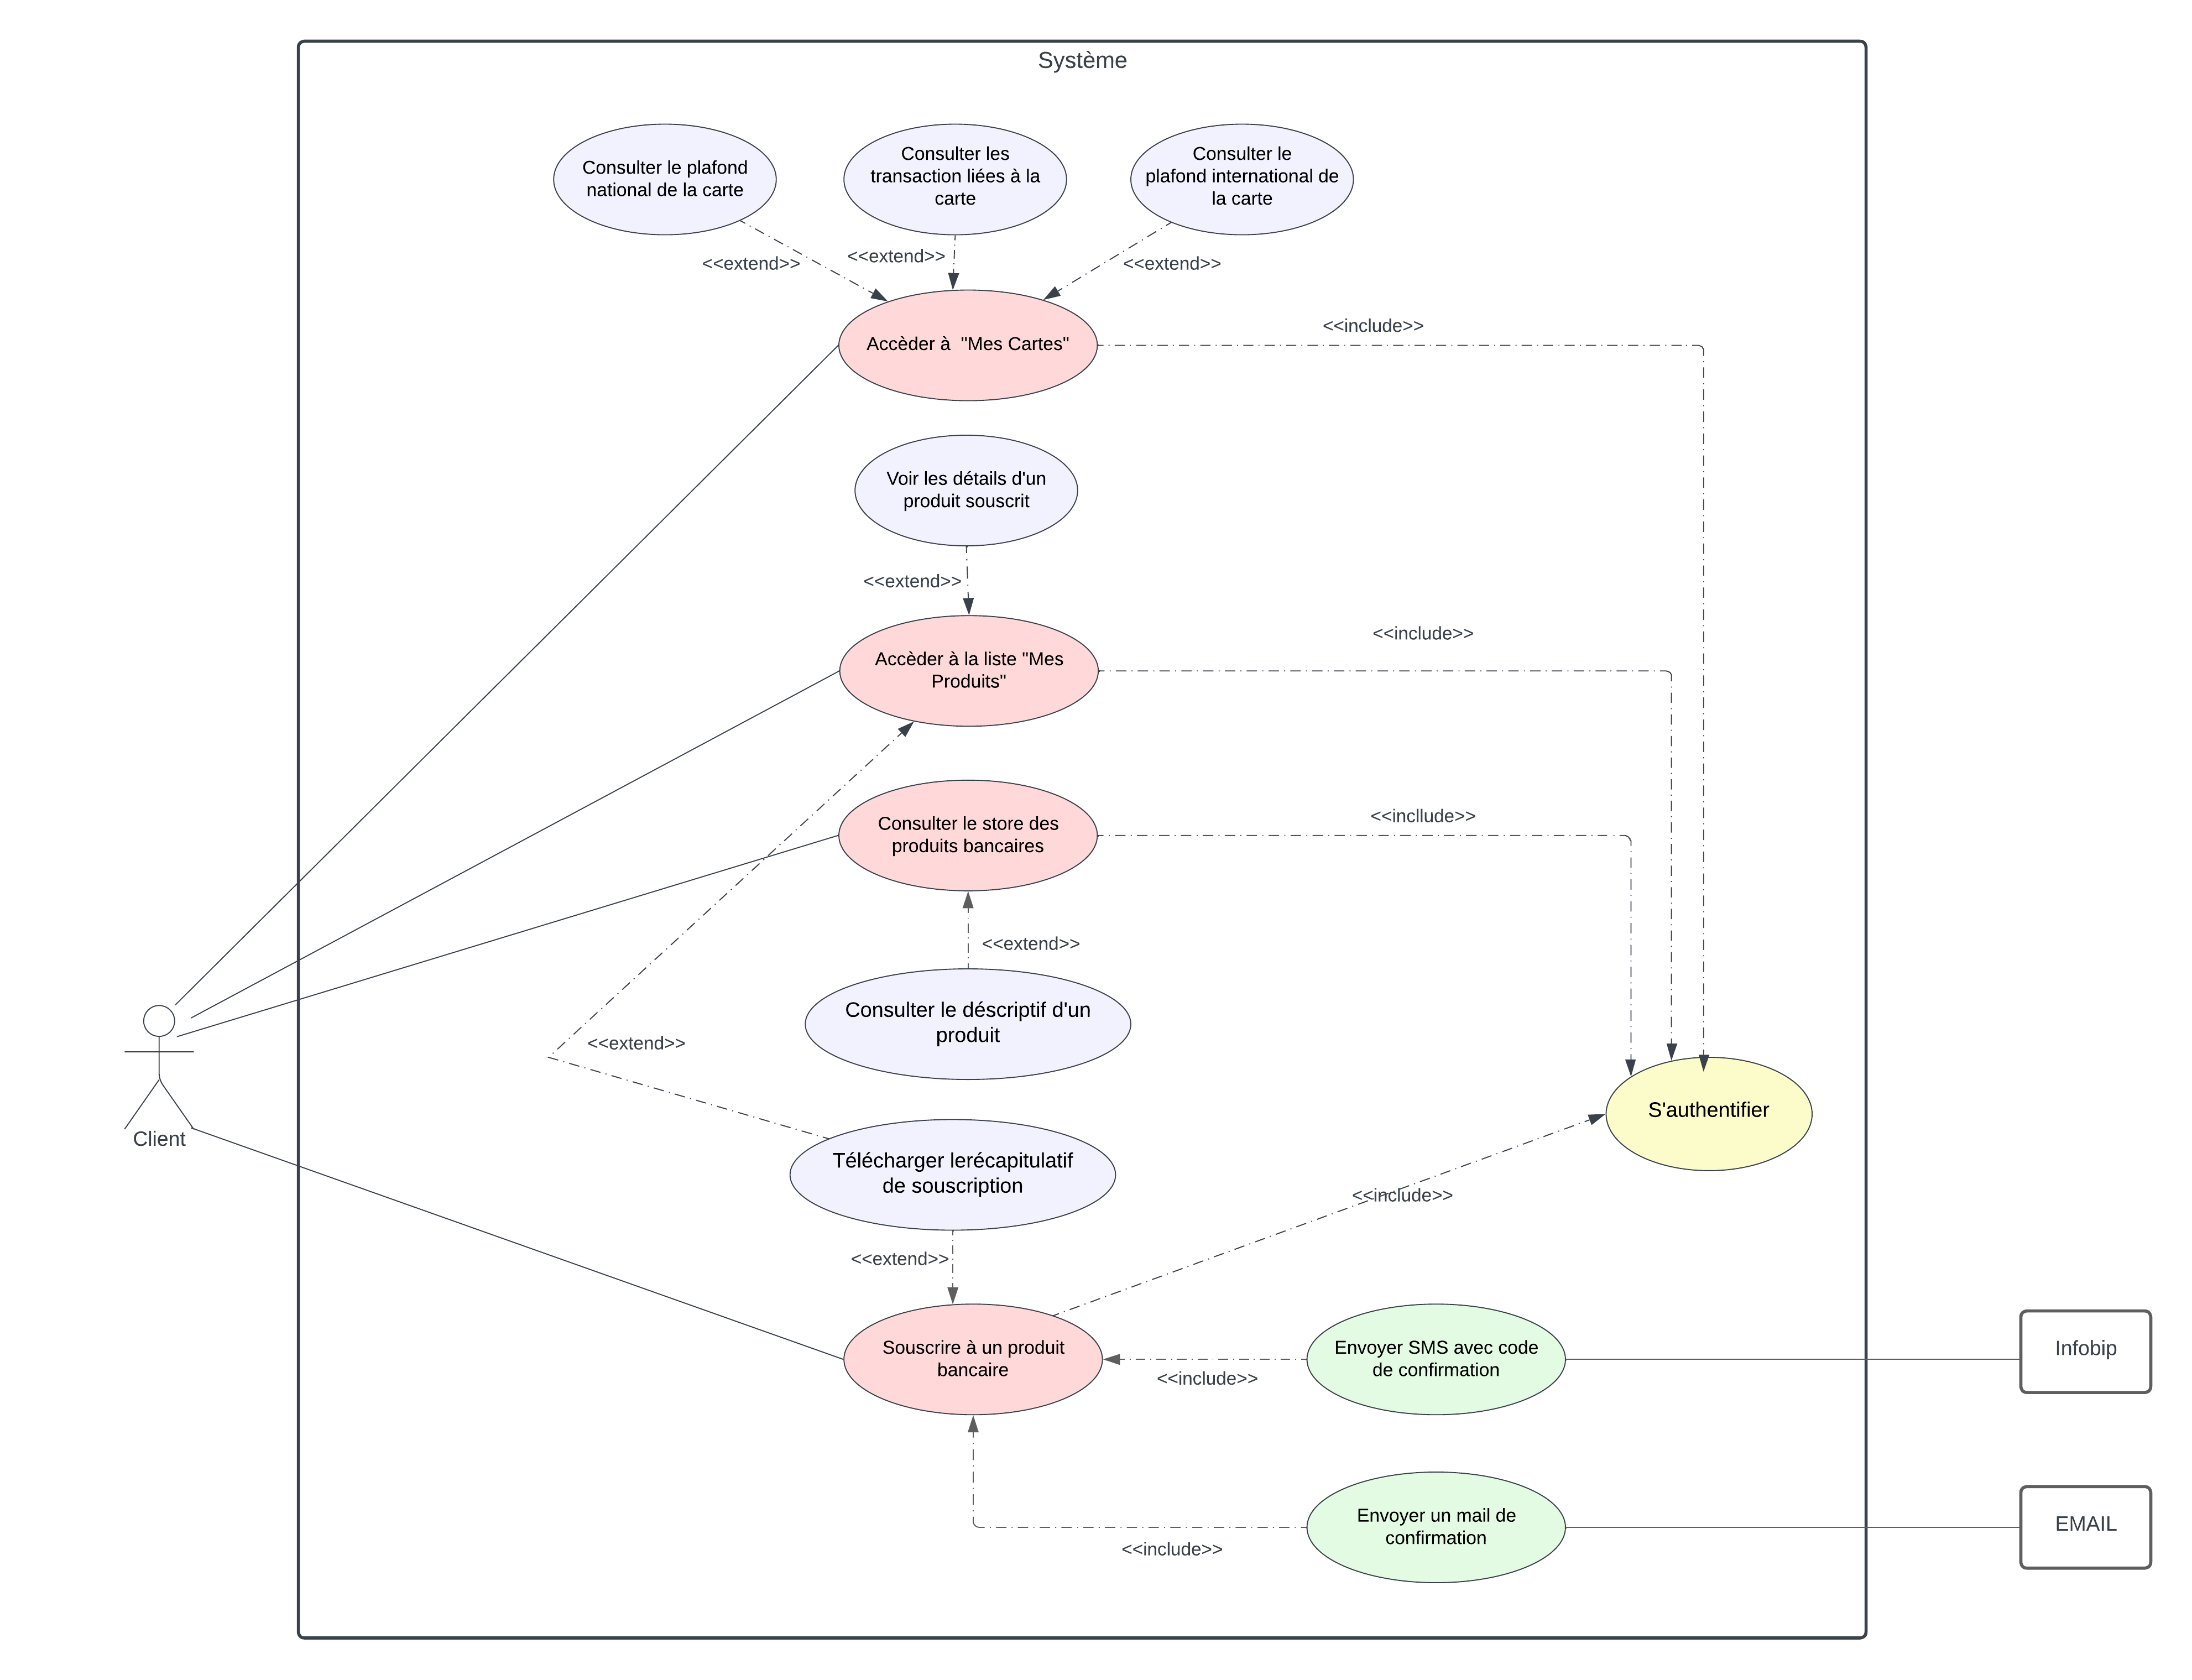
\includegraphics[width=16cm]{images/diagramms/useCase.png}
    \caption{Diagramme de cas d'utilisation}
\end{figure}
\newpage

Dans le diagramme de cas d'utilisation de notre système, nous avons les acteurs suivants :

\begin{itemize}
    \item[•] \textbf{Client :}  Représente l'utilisateur final, c'est-à-dire le client de la banque qui utilise l'application SG CONNECT pour accéder aux fonctionnalités bancaires disponibles.
    \item[•] \textbf{Infobip :} Système tiers qui joue le rôle de fournisseur de services d'envoi de SMS. Il est responsable du traitement des demandes d'envoi de SMS provenant de l'application SG CONNECT et de l'envoi des notifications SMS aux utilisateurs.
    \item[•] \textbf{EMAIL :} Système tiers qui gère l'envoi de notifications par courrier électronique aux utilisateurs. Il est utilisé pour informer les utilisateurs des opérations exécutées sur leur compte bancaire et pour partager l'historique des transactions, par exemple.
\end{itemize}

Ces acteurs interagissent avec le système SG CONNECT pour accéder aux fonctionnalités offertes et bénéficier des services bancaires à distance de manière sécurisée et pratique. Le client utilise l'application pour consulter ses comptes, effectuer des transactions, gérer ses cartes monétiques, etc. Infobip et EMAIL interviennent pour faciliter la communication avec les utilisateurs via des notifications SMS et des courriers électroniques.\\

Il est important de noter que dans ce diagramme de cas d'utilisation, le client est le principal acteur qui interagit directement avec le système, tandis que Infobip et EMAIL sont des acteurs externes qui fournissent des services de communication complémentaires.\\

\textbf{\large{Description des cas d’utilisations :}\\}

\textbf{Accéder à "Mes Cartes"} : Ce cas d'utilisation permet au client d'accéder à la liste de ses cartes monétiques associées à ses comptes bancaires. Le client peut consulter le plafond national ou international de chaque carte et afficher les transactions liées à chaque carte.\\

\textbf{Accéder à la liste "Mes Produits"} : Ce cas d'utilisation permet au client d'accéder à la liste des produits bancaires qu'il a souscrits. Le client peut voir les détails d'un produit souscrit spécifique et télécharger un récapitulatif de souscription pour référence.\\

\textbf{Consulter le store des produits bancaires} : Ce cas d'utilisation permet au client de consulter le catalogue des produits bancaires disponibles. Le client peut consulter le descriptif de chaque produit pour obtenir des informations détaillées.\\

\textbf{Souscrire à un produit bancaire} : Ce cas d'utilisation permet au client de souscrire à un produit bancaire spécifique. Le client peut télécharger un récapitulatif de la souscription pour référence. Lors de la souscription, le système envoie un SMS avec un code de confirmation en utilisant le service d'Infobip, et envoie également un mail de confirmation en utilisant le service d'EMAIL.\\

Tous les cas d'utilisation nécessitent une authentification préalable du client pour garantir la sécurité et la confidentialité des données.

\section{Conclusion}
Ce chapitre a été consacré à une étude détaillée du projet, mettant l'accent sur la spécification des besoins et leur analyse approfondie. Nous avons identifié les besoins fonctionnels et non fonctionnels du système, en nous assurant de couvrir les différentes fonctionnalités nécessaires pour répondre aux attentes des utilisateurs. Le diagramme de cas d'utilisation a permis de représenter de manière visuelle les interactions entre les acteurs et le système, en mettant en évidence les différentes fonctionnalités offertes. Cette analyse approfondie des besoins servira de base solide pour la conception de l'architecture du système, qui sera abordée dans le prochain chapitre. En concevant clairement l'architecture, nous pourrons garantir que le système répondra de manière efficace et satisfaisante aux besoins identifiés dans cette étude détaillée.